\documentclass{article}

\usepackage[utf8]{inputenc}
\usepackage[T1]{fontenc}
\usepackage{microtype}

\usepackage{newspaper}
%% [LianTze] Contains some modifications
\usepackage{newspaper-mod}
%%... so now you can redefine the headline and byline style if you want to.
%% These can be issued just before any
%% byline or headline in the paper, to
%% individually style each article
%%
% \renewcommand{\headlinestyle}{\itshape\Large\lsstyle}
% \renewcommand{\bylinestyle}{\bfseries\Large\raggedright}


\date{\today}
\currentissue{2}

%% [LianTze] The newspaper package also provides 
%% these commands to set various metadata:

%% The banner headline on the first page
%%   (The colon after s: is to get a more
%%   modern majuscule s in this font instead of 
%%   the medieval tall s. For anyone interested 
%%   in the history: 
%%  http://medievalwriting.50megs.com/scripts/letters/historys.htm)
\SetPaperName{Transformation news:}

%% The name used in the running header after
%% the first page
\SetHeaderName{Transformation news}

%% and also...
\SetPaperLocation{The Guild}
\SetPaperSlogan{``Ура, товарищи, грядёт!''}
\SetPaperPrice{Zero dollars}


% [LianTze] times (the package not the font) is rather outdated now; use newtx (see later)
% \usepackage{times}
\usepackage{graphicx}
\usepackage{wrapfig}
\usepackage{multicol}

\usepackage{picinpar}
%uasage of picinpar:
%\begin{window}[1,l,\includegraphics{},caption]xxxxx\end{window}


%%%%%%%%%  Front matter   %%%%%%%%%%

\usepackage{lipsum}

\begin{document}

\maketitle

\begin{abstract}
\headline{\bf\sf\Large ДОменный МЕНТОР - апологет качественного кода.}

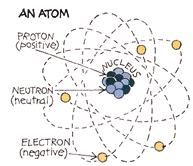
\includegraphics[]{atom.jpg}

Пробуем разобраться.
Подробности на странице 2.
\vspace{10mm}
\closearticle

\end{abstract}

\begin{multicols}{3}

\headline{\bf\sf\Large Поставки на бой станут регулярными, обеспечит ли это нам победу?}
Пробуем разобраться.
Подробности на странице 2.
\vspace{5mm}
\closearticle

\headline{\bf\sf\Large Волнение в правом крыле}
Разработчики выступают с лозунгом "Мы готовы жечь декларации Jenkins в своих репозиториях если наши требования по CICD не будут выполнены".
Подробности на странице 2.
\vspace{5mm}
\closearticle

\headline{\bf\sf\Large Принцип Эскобара и выбор механизма поставки.}
Как они связаны? Отвечает представитель левого крыла трансформации.
Подробности на странице 2.
\closearticle

\end{multicols}

\begin{multicols}{3}

\headline{\bf\sf\Large Jenkins. Как эксплуатация труда машин становится трендом.}
Комментарии идеолога.
Подробности на странице 2.
\closearticle

\headline{\bf\sf\Large Артефакт это не только продукт языческого культа!}
Статья известного архитектолога.
Подробности на странице 2.
\vspace{5mm}
\closearticle

\headline{\bf\sf\Large Почему артефакт нельзя передавать из рук в руки.}
Суеверие или современная концепция разработки. Пробуем разобраться.
Подробности на странице 2.
\closearticle

\end{multicols}

\begin{multicols}{3}

\headline{\bf\sf\normalsize "Они пришли и все началось", "Без них было лучше, зачем они пришли?", "Наше будущее смутно!".}
Головные боли и методы их лечения.
Подробности на странице 2.
\vspace{0mm}
\closearticle

\headline{\bf\sf\Large Игровые новости: Почему Morrowind снова захватывает мысли геймеров.}
Подробности на странице 2.
\vspace{30mm}
\closearticle

\end{multicols}

\end{document}